\documentclass[12pt, a4]{article}
\usepackage[english]{babel}
\usepackage[utf8]{inputenc}
\usepackage{fullpage}
\usepackage{listings}
\usepackage{graphicx}
\usepackage{color}

%Syntax highlighting
\definecolor{blue-violet}{rgb}{0.54, 0.17, 0.89}
\definecolor{ao}{rgb}{0.0, 0.5, 0.0}
\definecolor{amaranth}{rgb}{0.9, 0.17, 0.31}
\definecolor{ballblue}{rgb}{0.13, 0.67, 0.8}
\definecolor{onyx}{rgb}{0.06, 0.06, 0.06}


\lstset{
  breaklines=true,                 % automatic line breaking only at whitespace
  captionpos=b,                    % sets the caption-position to bottom
  breakatwhitespace=false,
  keepspaces=true,
  numbers=left,
  numbersep=5pt,
  showspaces=false,
  showstringspaces=false,
  showtabs=false,
  tabsize=4,  
  backgroundcolor=\color{white},   % choose the background color
  commentstyle=\color{ao},    % comment style
  keywordstyle=\color{amaranth},    % keyword style
  stringstyle=\color{blue-violet},    % string literal style
  numberstyle=\tiny\color{ballblue},	   % number style
  basicstyle=\ttfamily\footnotesize\color{onyx} % size of fonts used for the code
}


%Document Header
\title{\textbf{Department of CSE\\SSN College of Engineering}}
\author{\textbf{Vishakan Subramanian - 18 5001 196 - Semester VI}}
\date{13 February 2021}

\begin{document}
\maketitle
\hrule
\section*{\center{UCS 1611 - Internet Programming Lab}}
\hrule
\bigskip

%Assignment Details
\subsection*{\center{\textbf{Exercise 2: Website for International Conference using CSS}}}
\subsection*{\flushleft{Learning Objective:}}
\begin{flushleft}
To develop a Website for an International Conference using \textbf{HTML5 elements} with the following specifications:-

\begin{itemize}
\item While designing the web page:
\item Use Inline, Embedded, External Style Sheets.
\item Use box model, outline concepts.
\item CSS concepts with table, list, links, forms, anchor etc.
\item Write rules with rule cascading and inheritance.
\item Include Tooltip, Icons, Graphics, Animations, and Transformations.
\end{itemize}
 
\end{flushleft}

%Code
\newpage
\subsection*{\flushleft{Code - Home Page:}}
\begin{flushleft}
\lstinputlisting[language = HTML]{index.html}
\end{flushleft}

\newpage
\subsection*{\flushleft{Code - Committee Page:}}
\begin{flushleft}
\lstinputlisting[language = HTML]{committee.html}
\end{flushleft}

\newpage
\subsection*{\flushleft{Code - Call for Papers Page:}}
\begin{flushleft}
\lstinputlisting[language = HTML]{papers.html}
\end{flushleft}

\newpage
\subsection*{\flushleft{Code - Important Dates Page:}}
\begin{flushleft}
\lstinputlisting[language = HTML]{dates.html}
\end{flushleft}

\newpage
\subsection*{\flushleft{Code - Workshops Page:}}
\begin{flushleft}
\lstinputlisting[language = HTML]{workshops.html}
\end{flushleft}

\newpage
\subsection*{\flushleft{Code - Registration Page:}}
\begin{flushleft}
\lstinputlisting[language = HTML]{reg.html}
\end{flushleft}

\newpage
\subsection*{\flushleft{Code - Contact Page:}}
\begin{flushleft}
\lstinputlisting[language = HTML]{contact.html}
\end{flushleft}

\newpage
\subsection*{\flushleft{Code - Stylesheet:}}
\begin{flushleft}
\lstinputlisting[]{styles.css}
\end{flushleft}

%Output
\newpage
\subsection*{\flushleft{Output - Home Page:}}
\begin{figure}[h]
\centering
\caption{Browser Output: Home Page.}
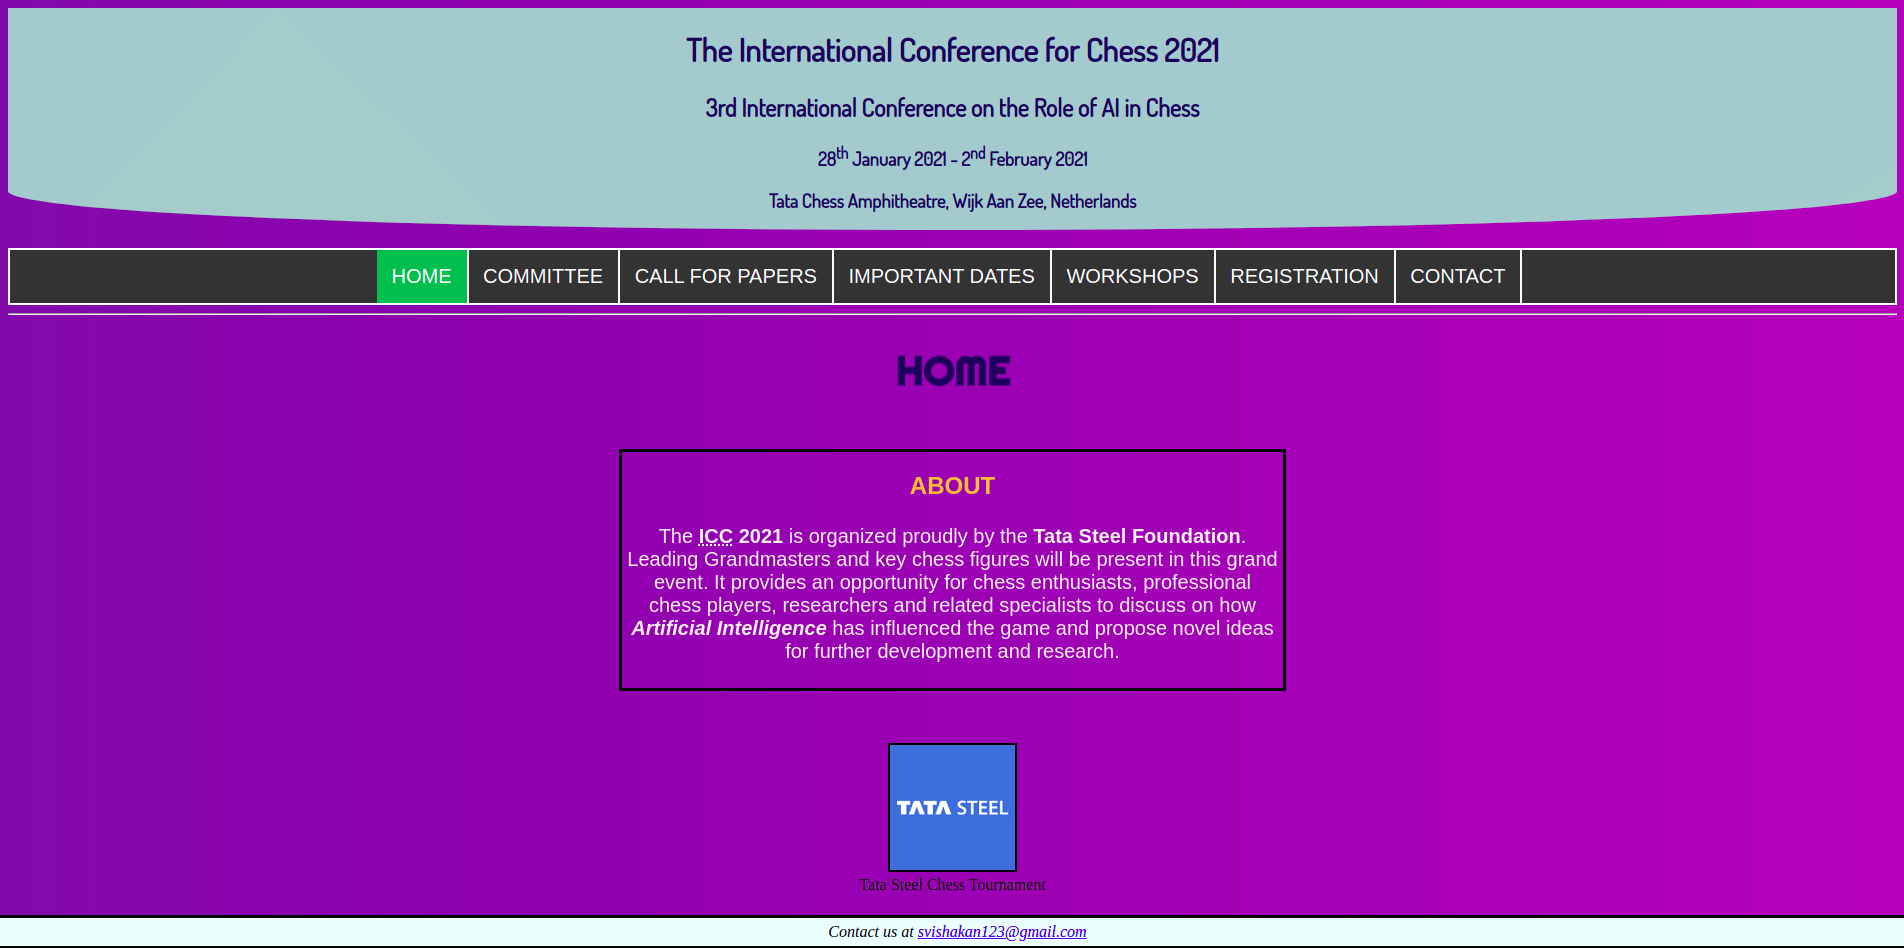
\includegraphics[height=10cm, width=18cm, keepaspectratio]{Output/Home.png}
\end{figure}

\newpage
\subsection*{\flushleft{Output - Committee Page:}}
\begin{figure}[h]
\centering
\caption{Browser Output: Committee Page.}
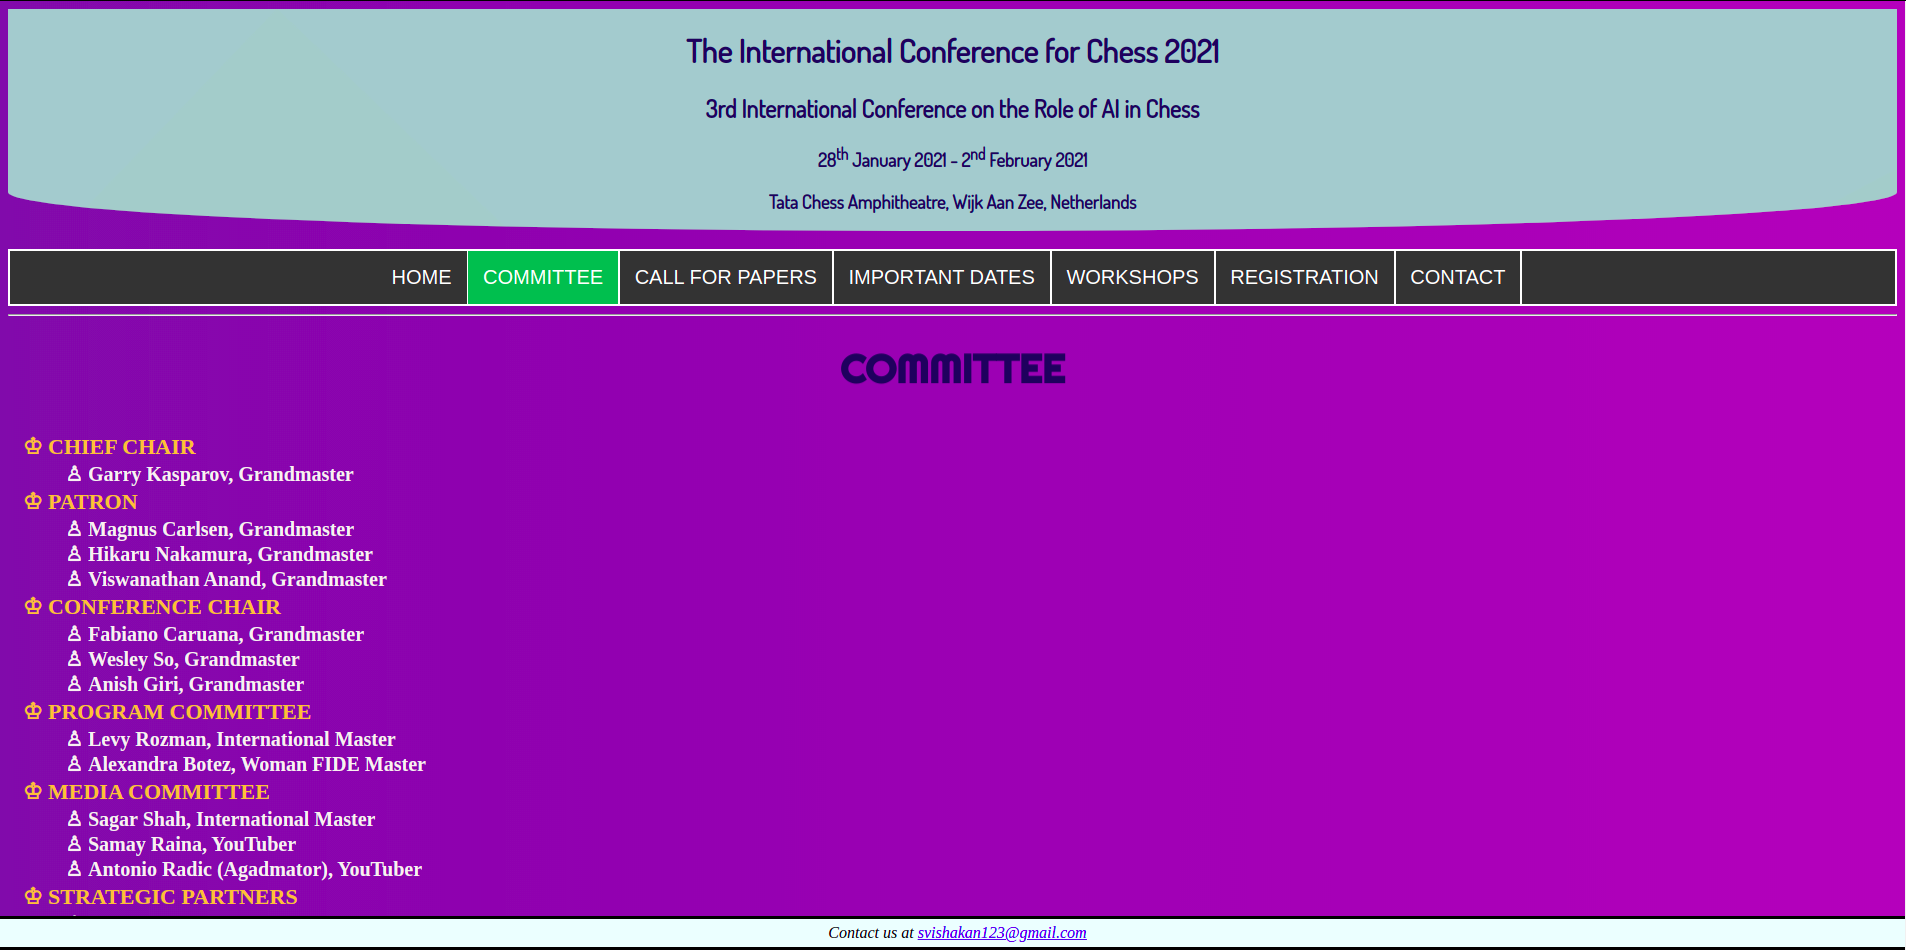
\includegraphics[height=10cm, width=18cm, keepaspectratio]{Output/Committee.png}
\end{figure}

\newpage
\subsection*{\flushleft{Output - Call For Papers Page:}}
\begin{figure}[h]
\centering
\caption{Browser Output: Call For Papers Page.}
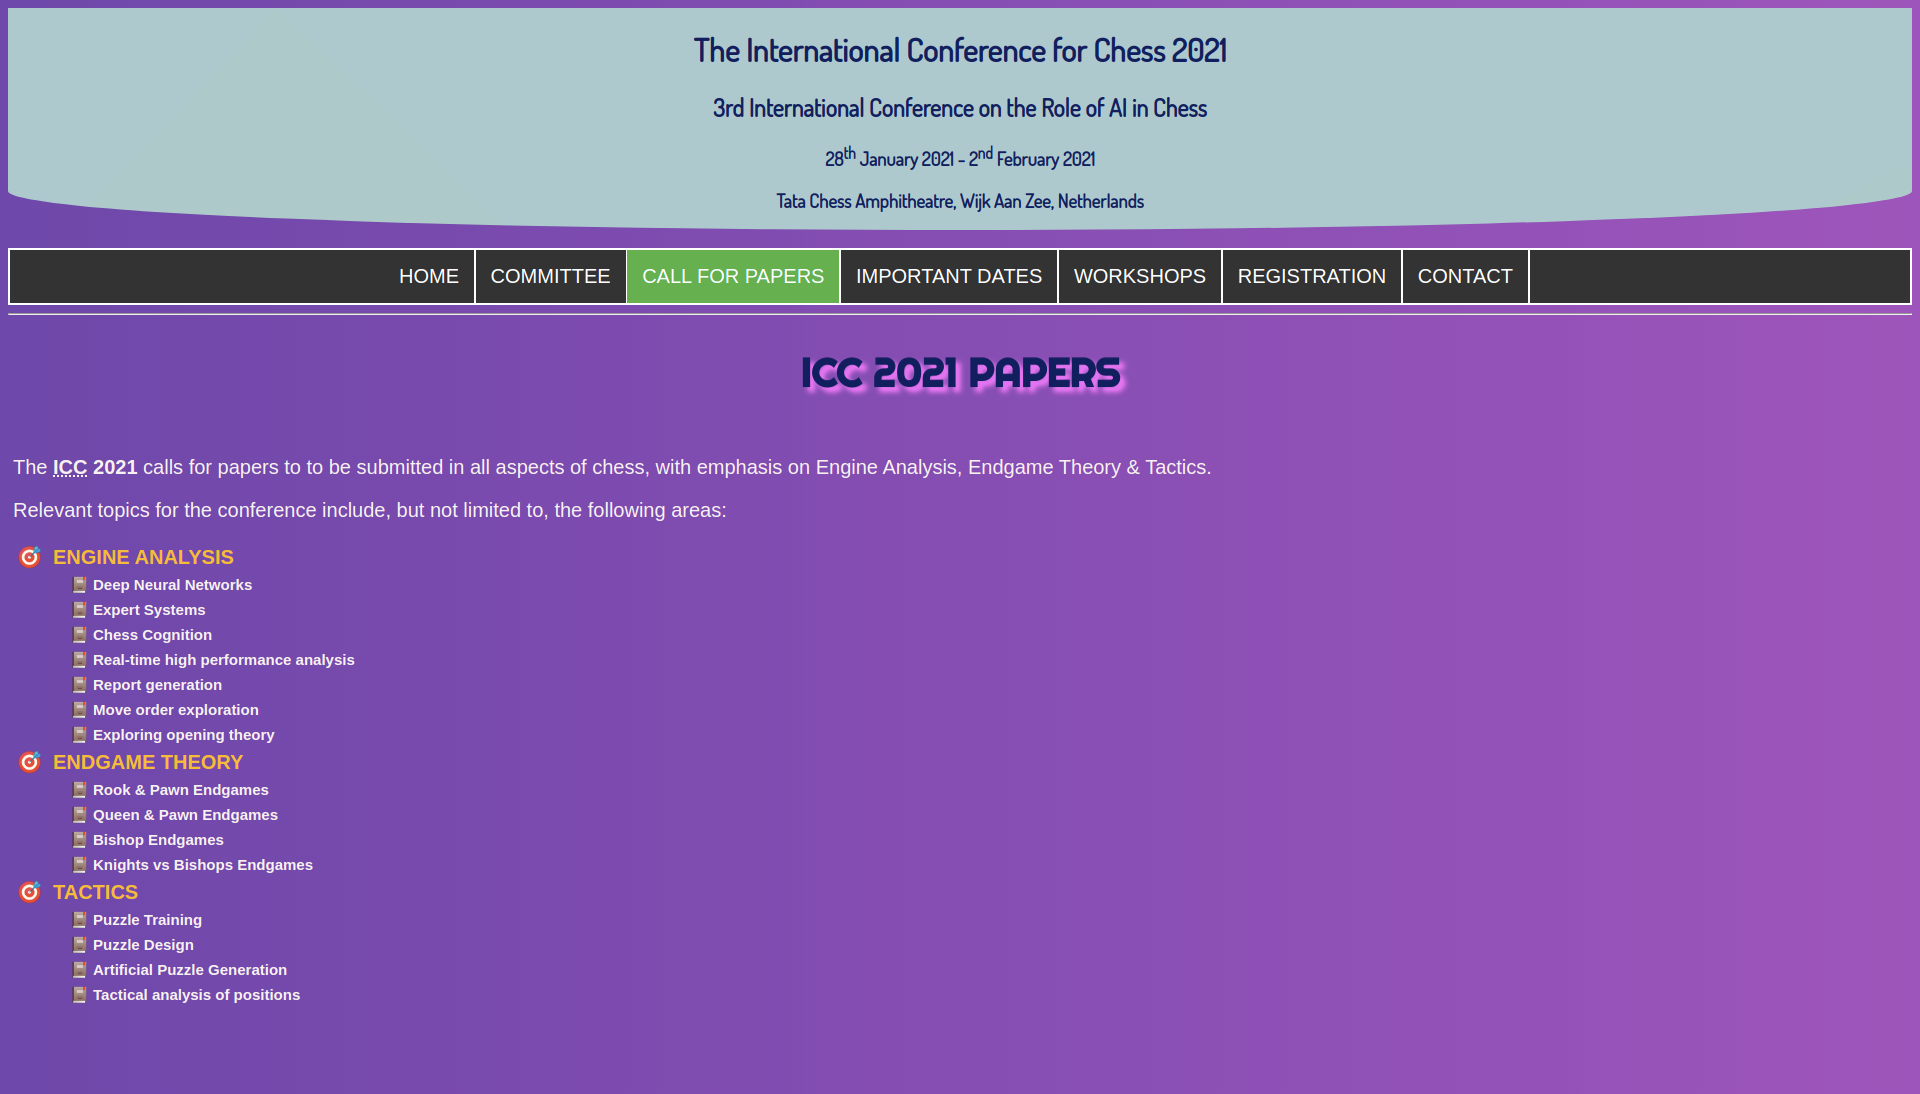
\includegraphics[height=10cm, width=18cm, keepaspectratio]{Output/Papers.png}
\end{figure}

\newpage
\subsection*{\flushleft{Output - Important Dates Page:}}
\begin{figure}[h]
\centering
\caption{Browser Output: Important Dates Page.}
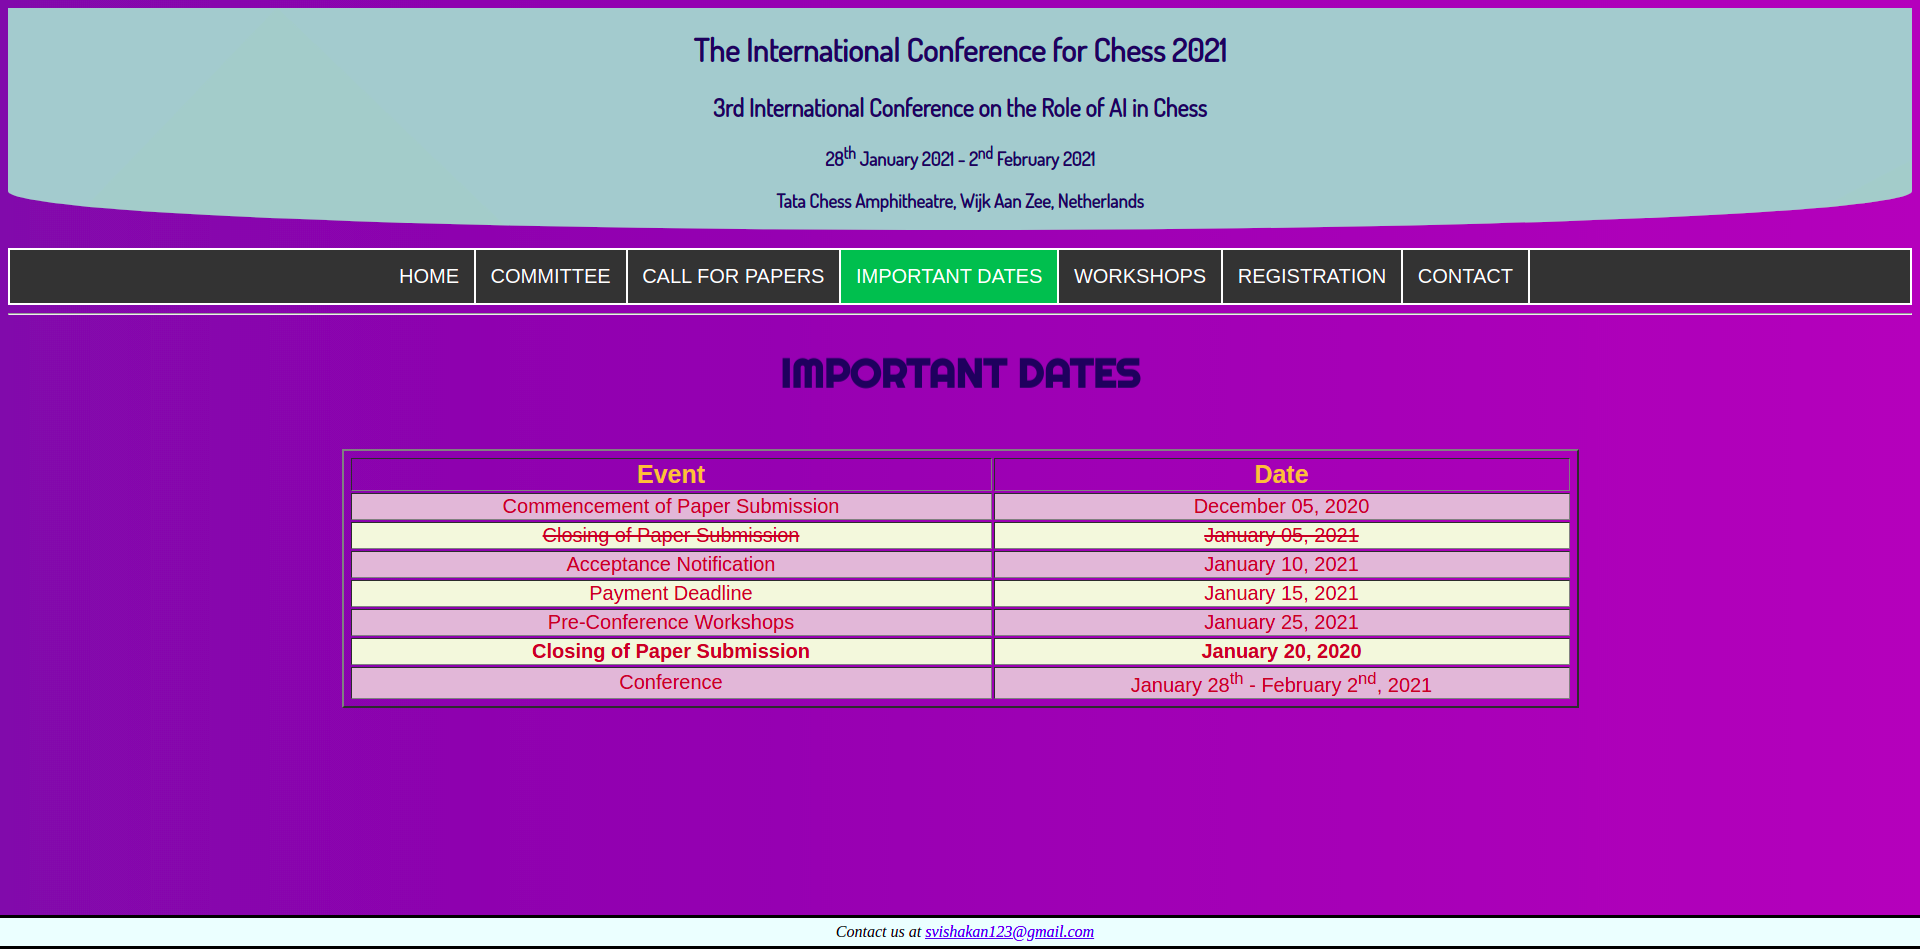
\includegraphics[height=10cm, width=18cm, keepaspectratio]{Output/Dates.png}
\end{figure}

\newpage
\subsection*{\flushleft{Output - Workshops Page:}}
\begin{figure}[h]
\centering
\caption{Browser Output: Workshops Page.}
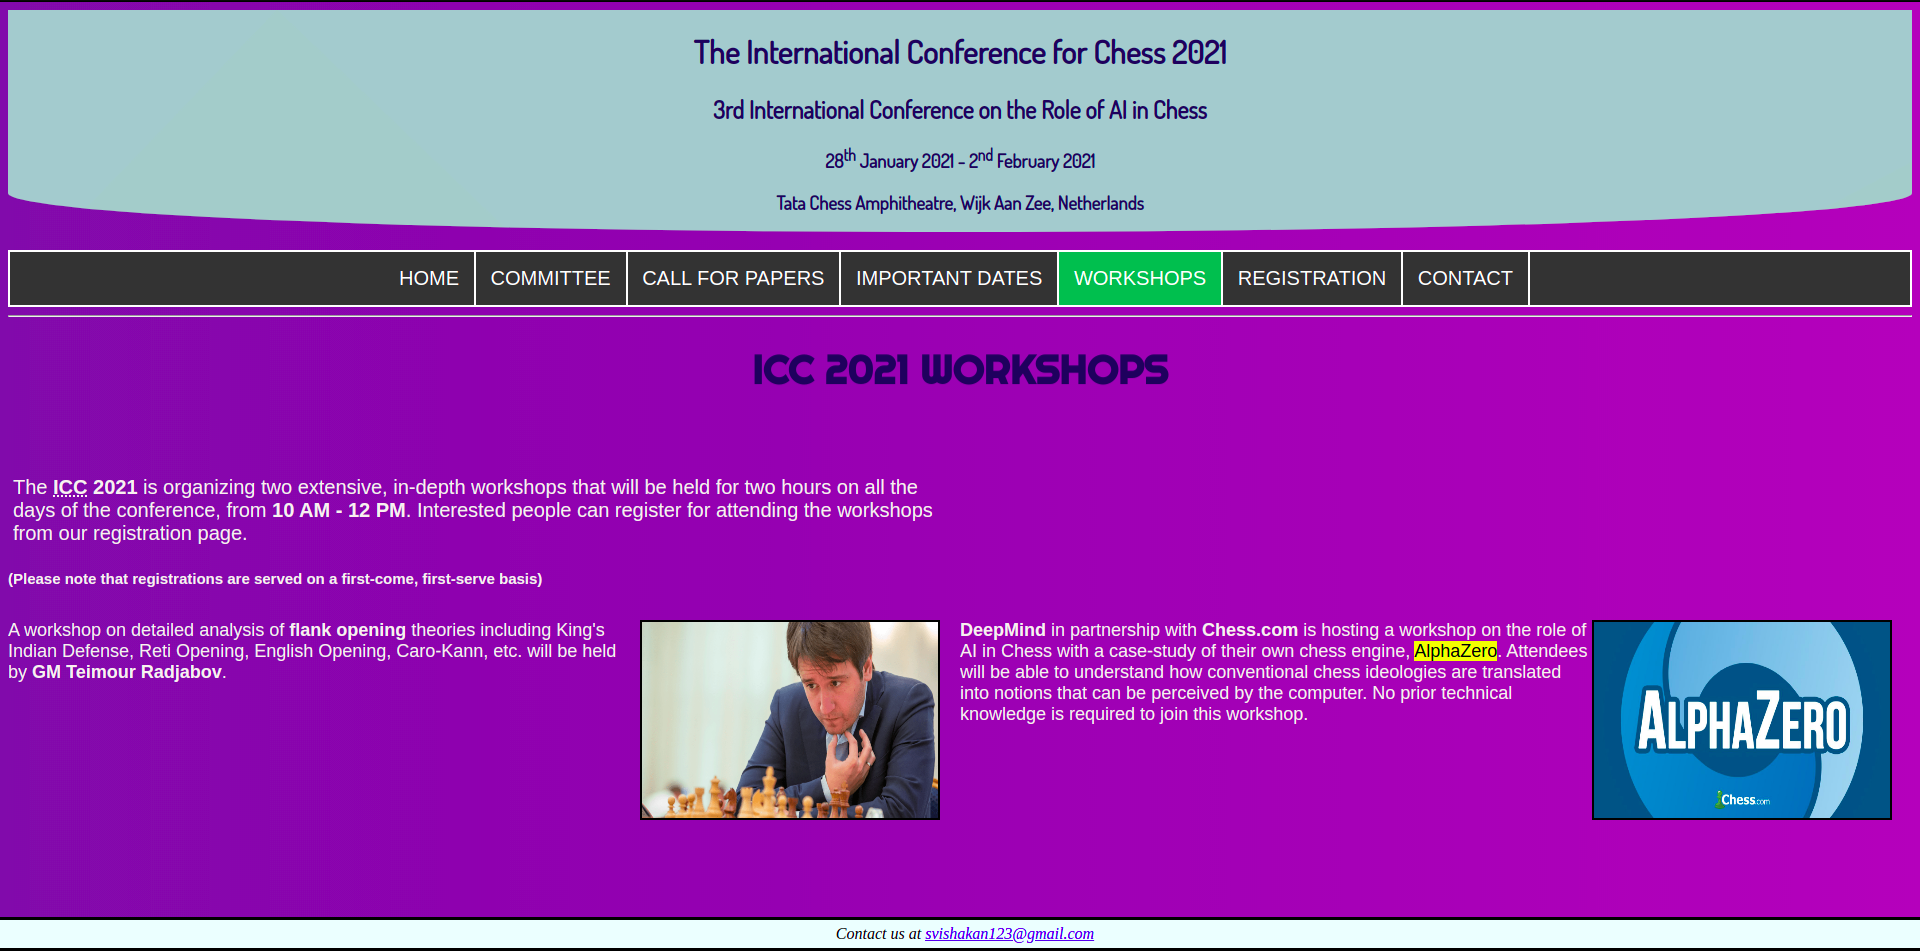
\includegraphics[height=10cm, width=18cm, keepaspectratio]{Output/Workshops.png}
\end{figure}

\newpage
\subsection*{\flushleft{Output - Registration Page:}}
\begin{figure}[h]
\centering
\caption{Browser Output: Registration Page.}
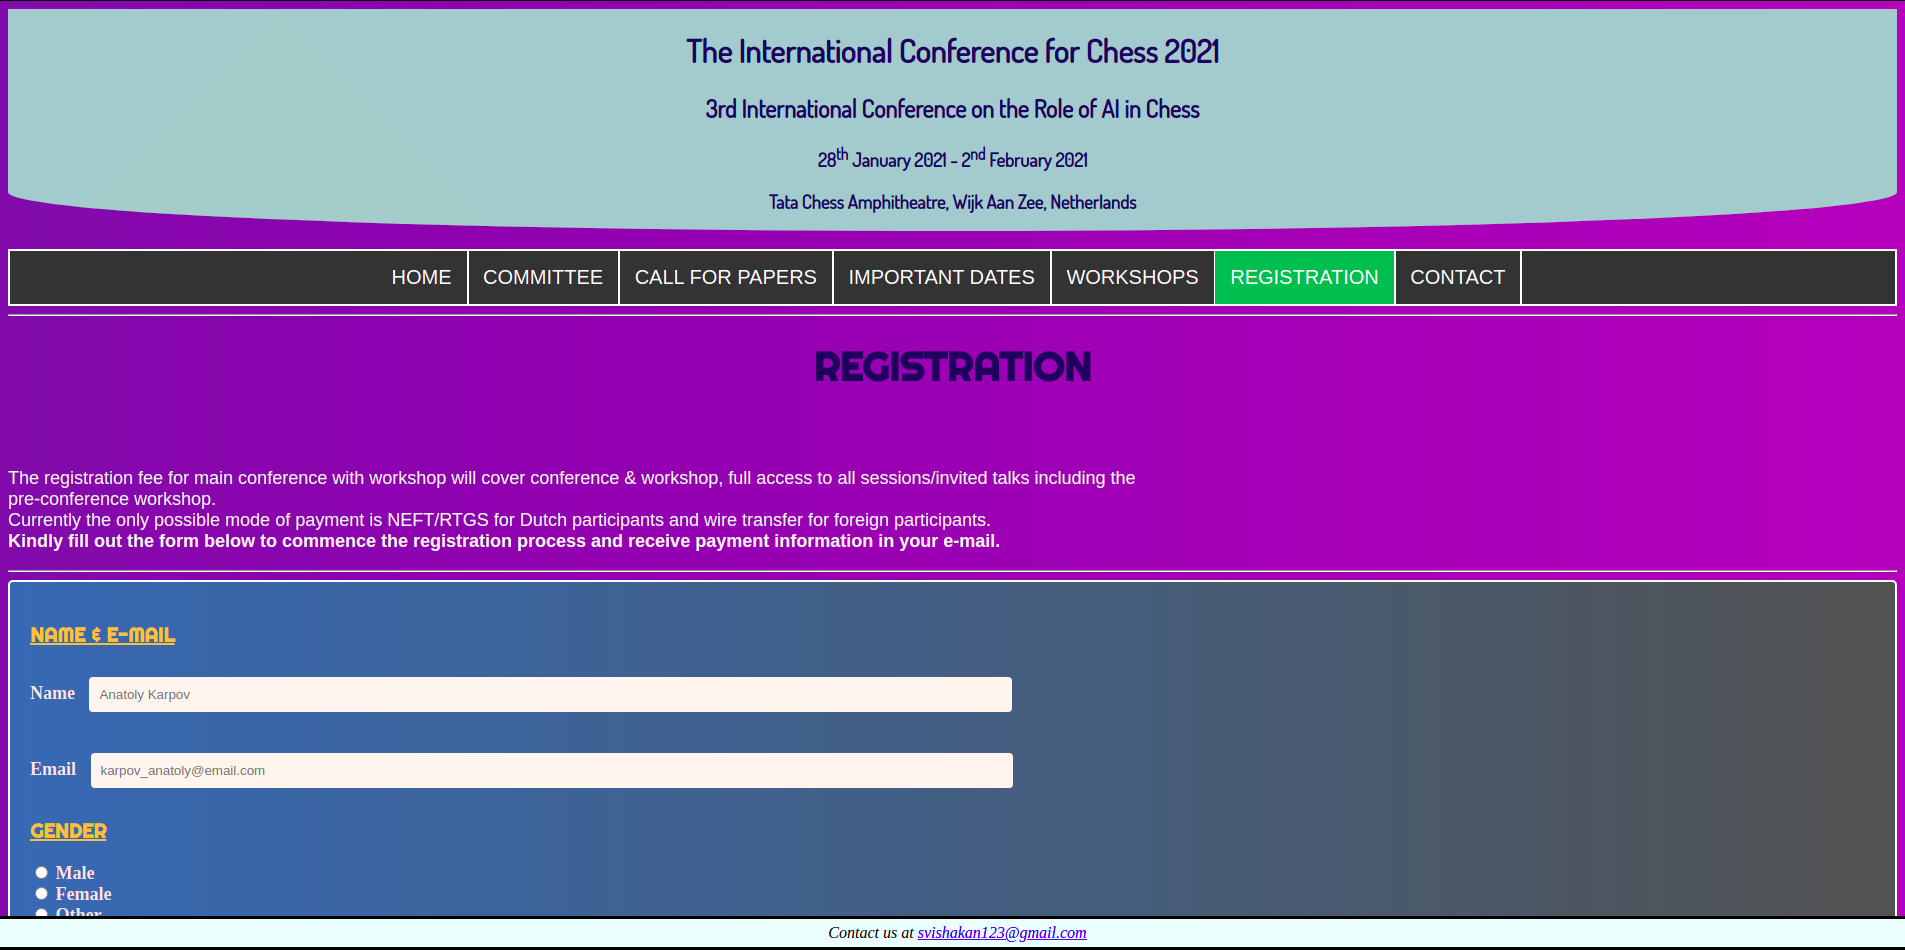
\includegraphics[height=10cm, width=18cm, keepaspectratio]{Output/Reg.png}
\end{figure}


\newpage
\subsection*{\flushleft{Output - Contact Page:}}
\begin{figure}[h]
\centering
\caption{Browser Output: Contact Page.}
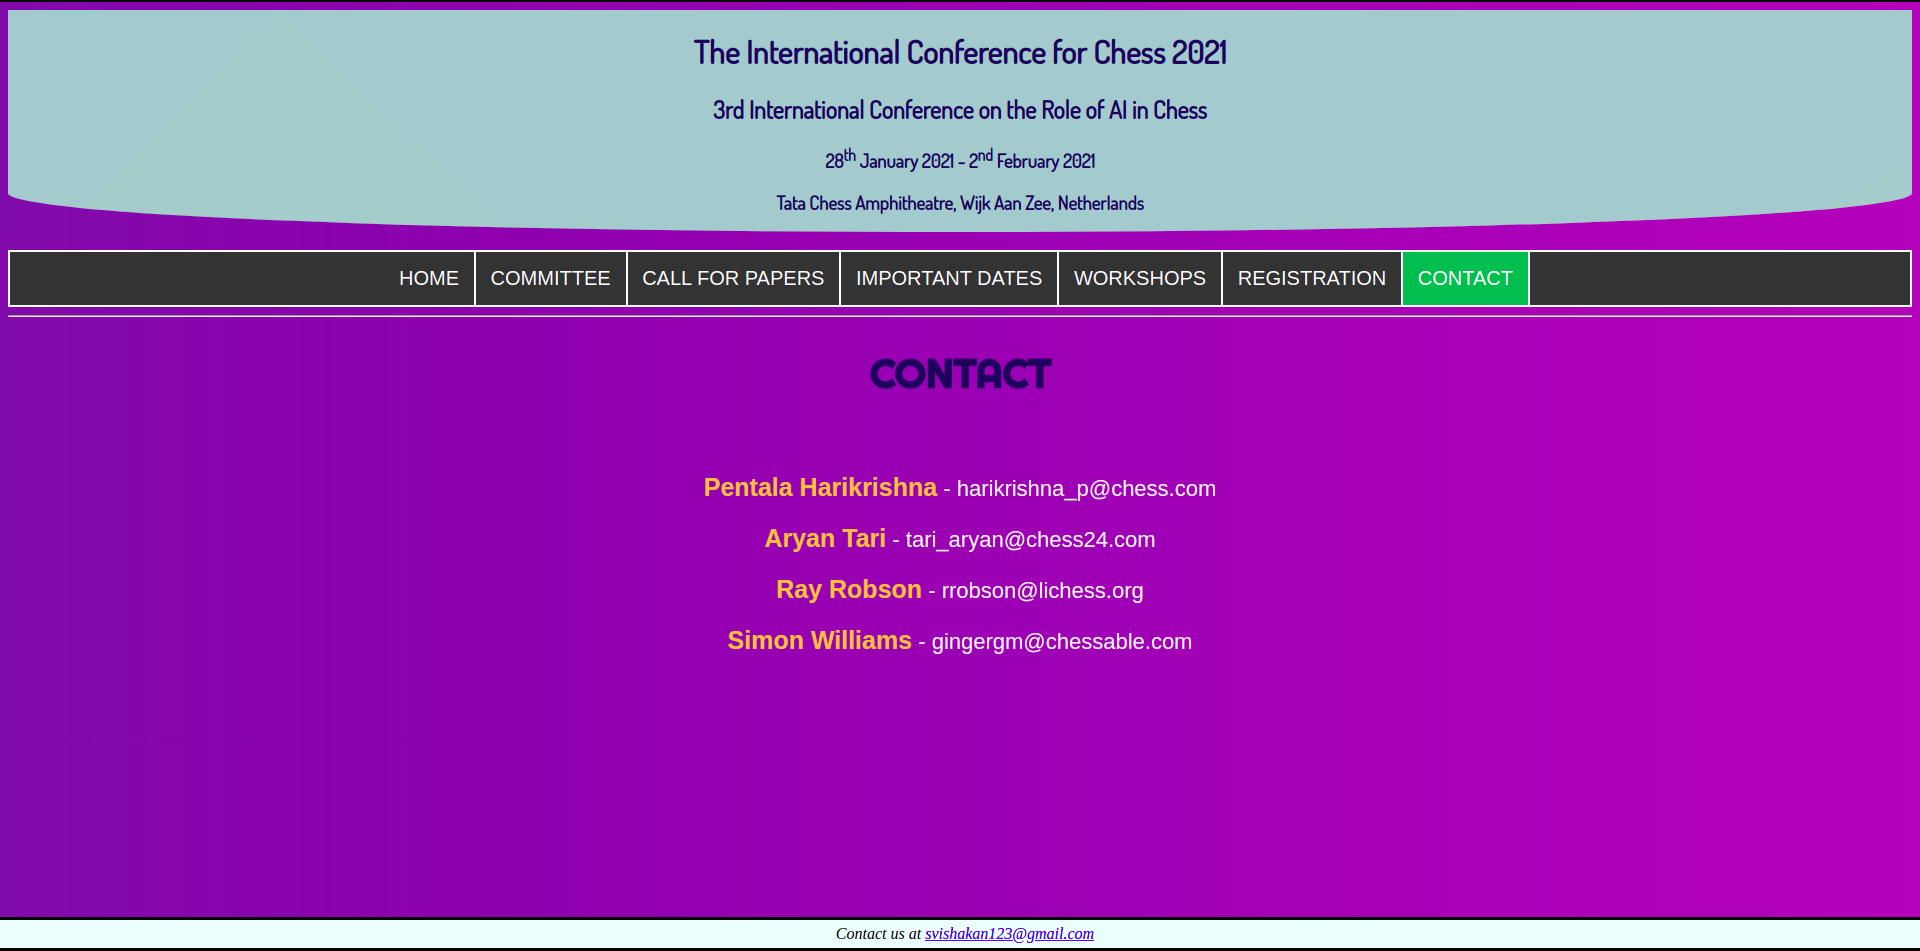
\includegraphics[height=10cm, width=18cm, keepaspectratio]{Output/Contact.png}
\end{figure}

%Learning Outcome
\newpage
\subsection*{\flushleft{Learning Outcome:}}
\begin{itemize}

\item From the experiment, I learnt to implement simple CSS tags.
\item I learnt about some common CSS attributes that can be used for most HTML tags like color, background-color, margin, padding etc.
\item I learnt how to do inline, internal and external CSS.
\item I learnt about selector based psuedo-class CSS tags like :hover, :nth-child, :active, :visited and their usage for anchor and table elements.
\item I was able to implement CSS for navigation bar, footer, tables and forms.
\item I learnt how to style different HTML elements.
\item I learnt to implement basic text animations and transitions.
\item I learnt and implemented various semantic tags of HTML5.
\item I learnt about implementing CSS by ID, tag type, class name and inheritance properties of CSS.
\item I learnt about different CSS selectors.
\item I learnt how to use icons for styling the bullet for unordered lists.
\item I learnt to import and use custom Google Fonts for styling the webpage.
\item I learnt and implemented basic box-modeling concepts, and understood about outlines, borders \& paddings in CSS.

\end{itemize}

\end{document}
